%%%%%%%%%%%%%%%%%%%%%%%%%%% Figure 8 The curvilinear grid %%%%%%%%%%%%%%%%%%%%
\begin{figure}[t]
 \begin{center}
  \begin{pspicture}(0,0)(15,8)
% Include graphs
   \rput[bl]( 0.0,0.0){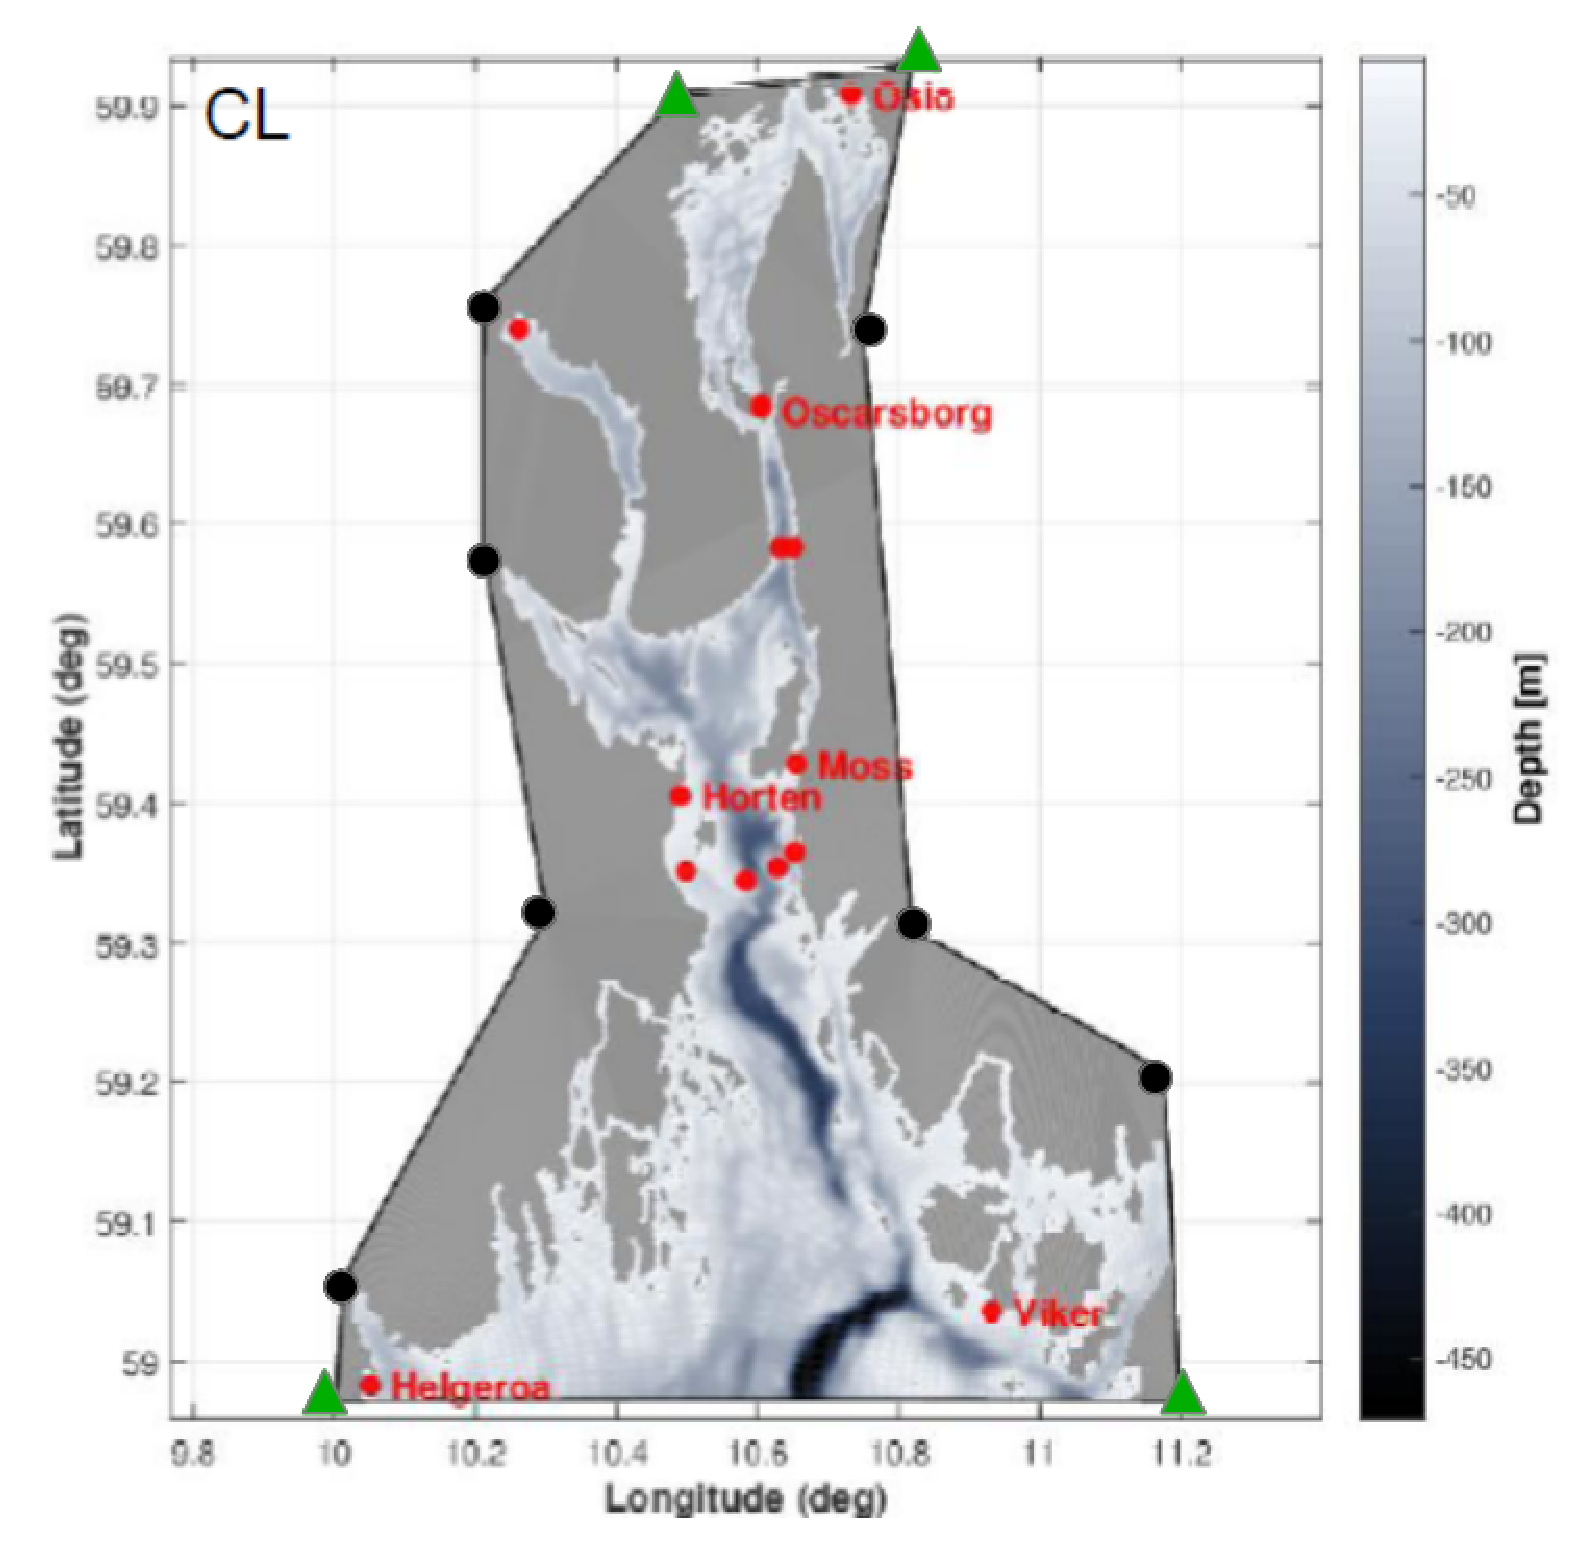
\includegraphics[height=8cm]{fjordos_nodes2}}
   \rput[br](15.3,0.0){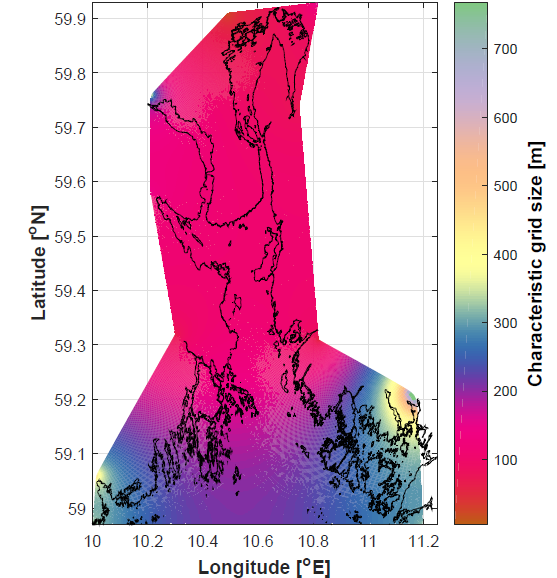
\includegraphics[height=7.82cm]{fjordos_grid}}
%   \rput[bl]( 0.0,0.0){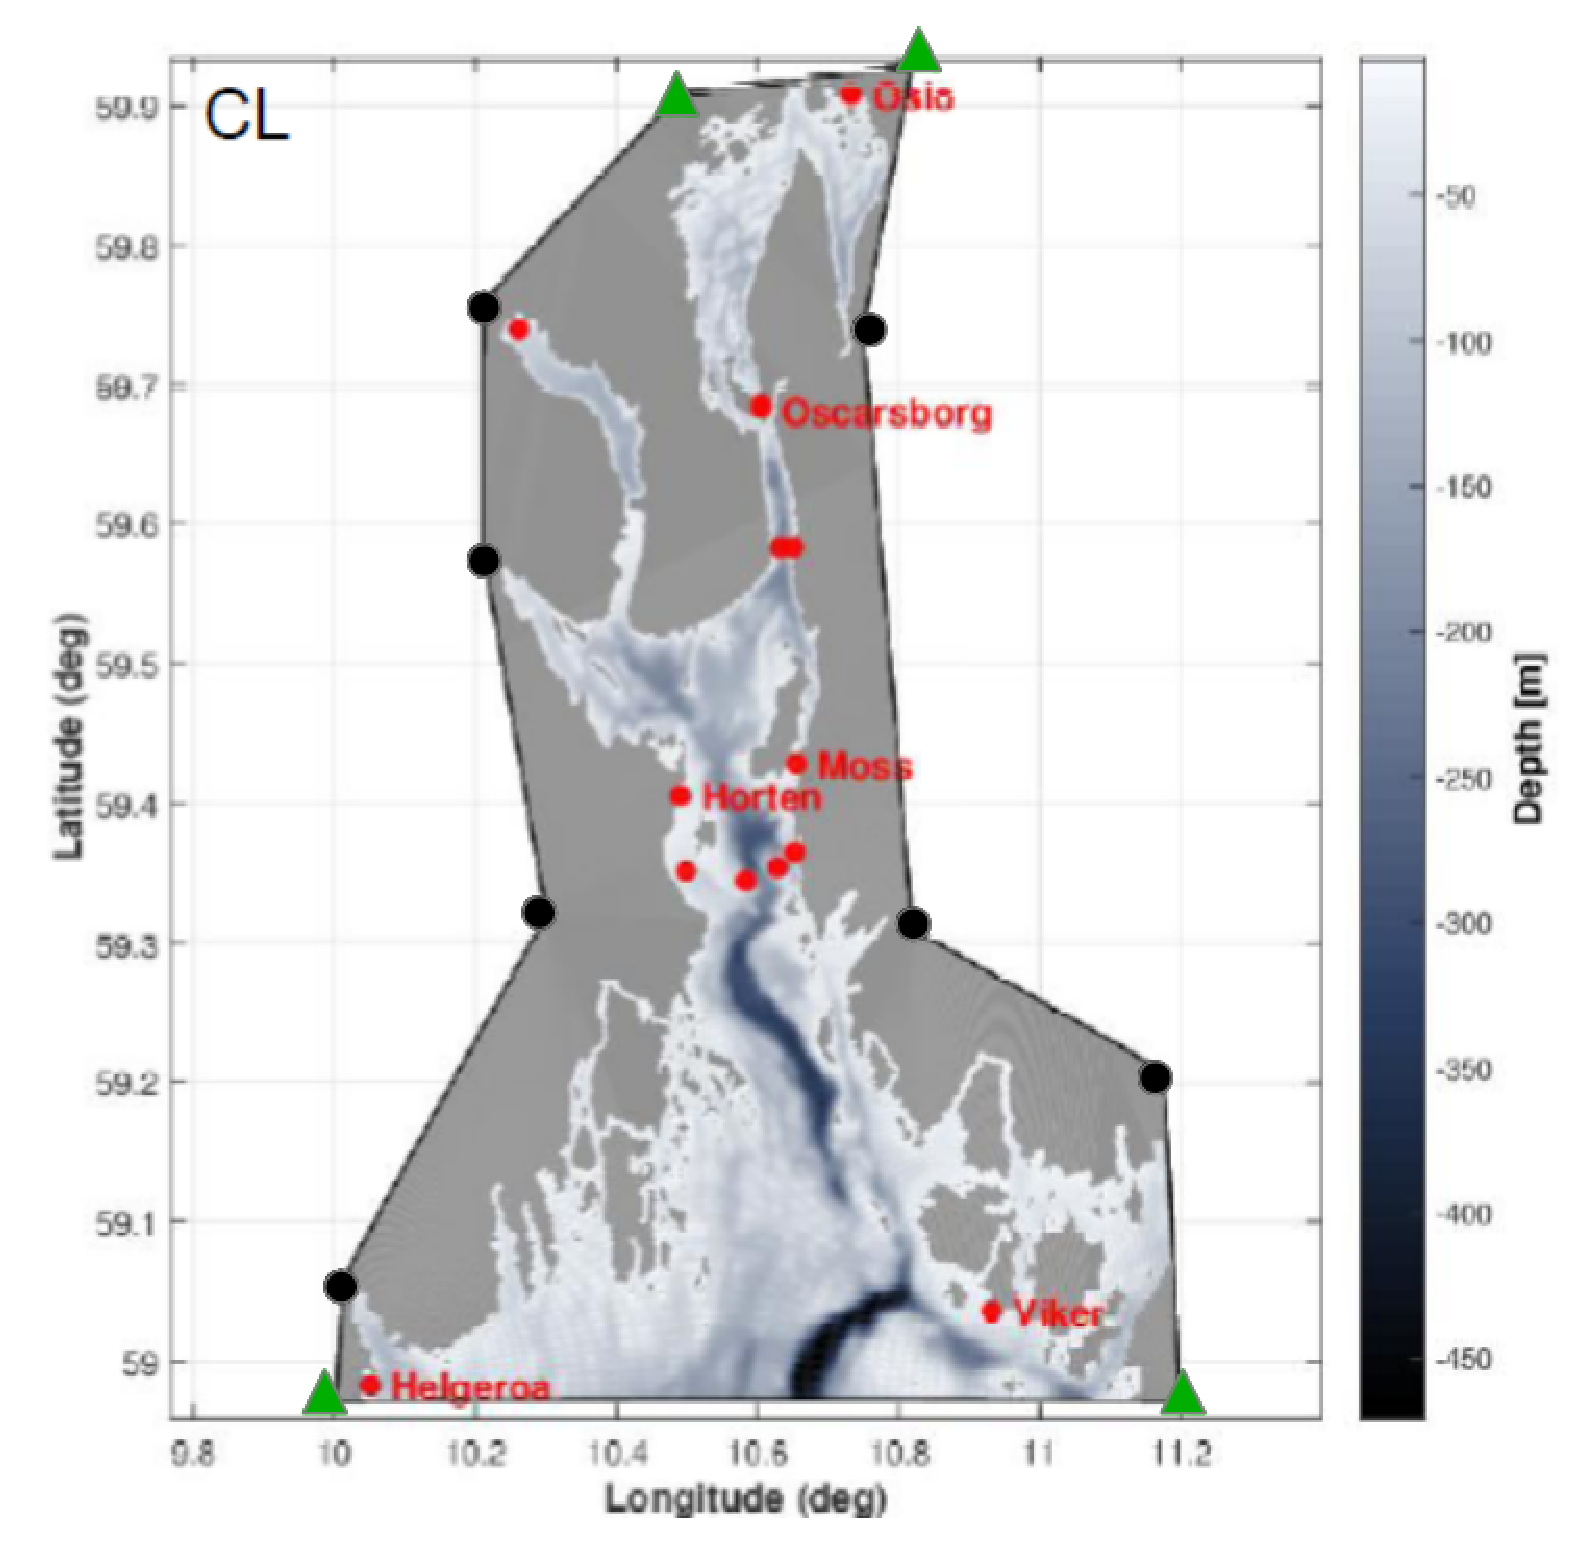
\includegraphics[width=7.8cm,height=9cm]{fjordos_nodes2}}
%   \rput[br](15.3,0.0){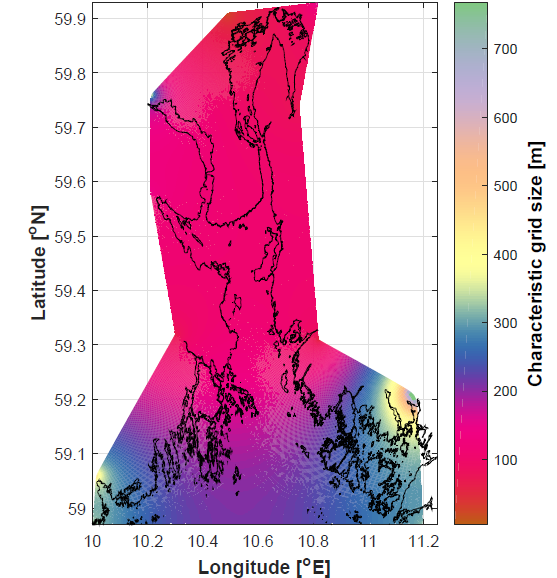
\includegraphics[width=8cm,height=8.8cm]{fjordos_grid}}
  \end{pspicture}
  \caption{\small Depicted are (a) the corners (green triangles) and nodes (black dots) determining the curvilinear grid for the new Oslofjord model, and (b) the resulting variable grid size. In (a) the depth in meters are indicated by the grayscale bar to the right, while the red dots indicate positions of well known places. In (b) the color bar indicates the grid's variable mesh size in meters.} 
  \label{fig:fjordos_grid}
 \end{center}
\end{figure}

